
On considère le programme de calcul suivant :

\begin{center}
	\begin{tikzpicture}[>=stealth]
		\node at  (0,10) {Choisir un nombre};
		\draw[shift={(0,8)}] (-1,-0.4) rectangle (1,0.4);
		\draw[shift={(-4.5,6)}] (-1,-0.4) rectangle (1,0.4);
		\draw[shift={(4.5,6)}] (-1,-0.4) rectangle (1,0.4);
		\draw[shift={(0,2)}] (-1,-0.4) rectangle (1,0.4) (0,-0.4) node[below] {Résultat final};
		\draw[->] (0,9.6)--(0,8.5);
		\draw[->] (0,7.6)--(-4.5,6.5) node[pos=0.4,left=5mm] {Soustraire 2};
		\draw[->] (0,7.6)--(4.5,6.5)node[pos=0.4, right=5mm] {Ajouter 1};
		\draw (-4.5,5.6)--(0,4) node[above=4mm,text width=4cm,align=center]{Multiplier les deux résultats}--(4.5,5.6);
		\draw[->] (0,4)--(0,2.5);
	\end{tikzpicture}
\end{center}

\textbf{Partie A}

\smallskip

\begin{enumerate}
	\item Justifier qu'en choisissant 5 comme nombre de départ, le résultat final obtenu est 18.

	\item Calculer le résultat final donné par ce programme lorsque le nombre de départ choisi est $-\dfrac{3}{2}$.

	\item Le script donné ci-dessous, écrit avec un logiciel de programmation, correspond au programme de calcul ci-dessus.


\begin{center}
\begin{scratch}[num blocks]
\blockinit{Quand \greenflag est cliqué}
\blocksensing{demander \ovalnum{choisir un nombre} et attendre}
\blockvariable{mettre \selectmenu{a} à \ovaloperator{\ovalsensing{réponse} - \ovalnum{\ldots}}}
\blockvariable{mettre \selectmenu{b} à \ovaloperator{\ovalsensing{réponse} + \ovalnum{\ldots}}}
\blocklook{dire \ovaloperator{\ovalnum{\ldots}*\ovalnum{\ldots}} pendant \ovalnum{2} secondes}
\end{scratch}
\end{center}

	Compléter les lignes 3, 4 et 5 du script ci-dessus, \textbf{à rendre avec la copie}. Aucune justification n'est attendue.
\end{enumerate}

\medskip

\textbf{Partie B}

\smallskip

Soit la fonction $g$ définie, pour un nombre $x$ donné, par $g(x) = x^{2}-x-2$.

\begin{enumerate}
	\item Prouver que $(x-2)(x+1)=x^{2}-x-2$.

	\item \begin{enumerate}
		\item Résoudre l'équation $(x-2)(x+1)=0$.
		\item En déduire les antécédents de 0 par la fonction $g$. Aucune justification n'est attendue.
	\end{enumerate}


	\item Parmi les trois graphiques ci-dessous, lequel correspond à la représentation graphique de la fonction $g$ ? Aucune justification n'est attendue.

	\begin{tblr}{colspec={X[c]X[c]X[c]}, vlines,hlines}
		Graphique 1 & Graphique 2 & Graphique 3\\
		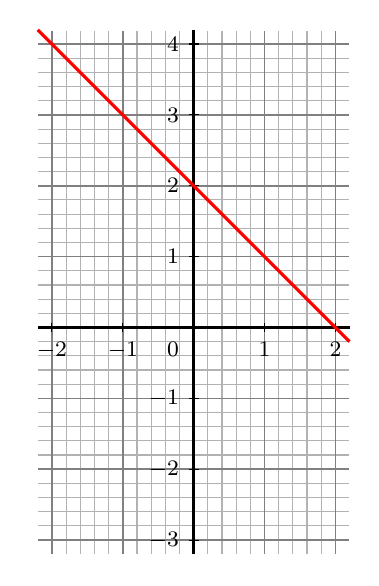
\begin{tikzpicture}[scale=0.9]%échelle originale : environ 1cm en x et en y
		\draw [color = gray!60, line width = 0.4pt, xstep=0.2, ystep = 0.2] (-2.19,-3.19) grid (2.19,4.19);
		\draw [color = gray, line width = 0.6pt, xstep=1, ystep = 1] (-2.19,-3.19) grid (2.19,4.19);
		\draw[line width=1pt] (-2.2,0) -- (2.2,0);
		\foreach \x in {-2,-1,1,2}{
		\draw[shift={(\x,0)},color=black] (0pt,2pt) -- (0pt,-2pt) node[below] {\footnotesize $\np{\x}$};
		}
		\draw[line width=1pt] (0,-3.2) -- (0,4.2);
		\foreach \y in {-3,-2,-1,1,2,3,4}{
		\draw[shift={(0,\y)},color=black] (2pt,0pt) -- (-2pt,0pt) node[left] {\footnotesize $\np{\y}$};
		}
		\draw[color=black] (-2pt,-2pt) node[below left] {\footnotesize 0};
		\draw[line width=1.2pt,color=red,smooth,samples=100,domain= -2.2:2.2 ] plot(\x,{2-\x} );
		\end{tikzpicture}&
		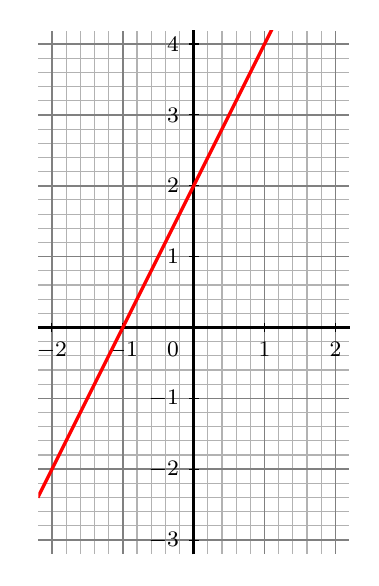
\begin{tikzpicture}[scale=0.9]%échelle originale : environ 1cm en x et en y
		\draw [color = gray!60, line width = 0.4pt, xstep=0.2, ystep = 0.2] (-2.19,-3.19) grid (2.19,4.19);
		\draw [color = gray, line width = 0.6pt, xstep=1, ystep = 1] (-2.19,-3.19) grid (2.19,4.19);
		\draw[line width=1pt] (-2.2,0) -- (2.2,0);
		\foreach \x in {-2,-1,1,2}{
		\draw[shift={(\x,0)},color=black] (0pt,2pt) -- (0pt,-2pt) node[below] {\footnotesize $\np{\x}$};
		}
		\draw[line width=1pt] (0,-3.2) -- (0,4.2);
		\foreach \y in {-3,-2,-1,1,2,3,4}{
		\draw[shift={(0,\y)},color=black] (2pt,0pt) -- (-2pt,0pt) node[left] {\footnotesize $\np{\y}$};
		}
		\draw[color=black] (-2pt,-2pt) node[below left] {\footnotesize 0};
		\clip (-2.19,-3.19) rectangle (2.19,4.19);
		\draw[line width=1.2pt,color=red,smooth,samples=100,domain= -2.2:1.2 ] plot(\x,{2*\x+2});
		\end{tikzpicture}&
		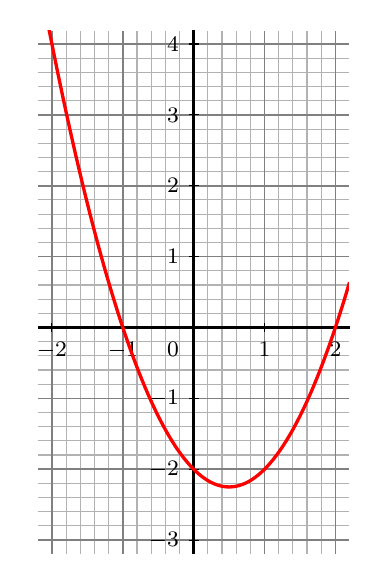
\begin{tikzpicture}[scale=0.9]%échelle originale : environ 1cm en x et en y
			\draw [color = gray!60, line width = 0.4pt, xstep=0.2, ystep = 0.2] (-2.19,-3.19) grid (2.19,4.19);
			\draw [color = gray, line width = 0.6pt, xstep=1, ystep = 1] (-2.19,-3.19) grid (2.19,4.19);
			\draw[line width=1pt] (-2.2,0) -- (2.2,0);
			\foreach \x in {-2,-1,1,2}{
			\draw[shift={(\x,0)},color=black] (0pt,2pt) -- (0pt,-2pt) node[below] {\footnotesize $\np{\x}$};
			}
			\draw[line width=1pt] (0,-3.2) -- (0,4.2);
			\foreach \y in {-3,-2,-1,1,2,3,4}{
			\draw[shift={(0,\y)},color=black] (2pt,0pt) -- (-2pt,0pt) node[left] {\footnotesize $\np{\y}$};
			}
			\draw[color=black] (-2pt,-2pt) node[below left] {\footnotesize 0};
			\clip (-2.19,-3.19) rectangle (2.19,4.19);
			\draw[line width=1.2pt,color=red,smooth,samples=100,domain=-2.2 :2.2 ] plot(\x,{\x*\x-\x-2});
		\end{tikzpicture}\\
	\end{tblr}
	\item Quel(s) nombre(s) doit-on choisir comme nombre de départ pour que le programme de calcul donne 0 comme résultat final ?
\end{enumerate}

\bigskip

